\documentclass[11pt]{article}
\usepackage[utf8]{inputenc}
\usepackage[T1]{fontenc}
\usepackage{amsmath,amssymb,amsthm}
\usepackage{mathtools}
\usepackage{graphicx}
\usepackage{booktabs}
\usepackage[margin=1in]{geometry}
\usepackage[hidelinks]{hyperref}
\usepackage{cmap}
\usepackage{xcolor}

\newcommand{\flag}[1]{\medskip\noindent\textcolor{red}{[\,#1\,]}\medskip}

\title{Identifying roughness from an option surface:\\
from a single smile to a live crypto market}
\author{Michael Lumor\thanks{Independent research programme; University of
Salford. ORCID: \href{https://orcid.org/0009-0000-0326-3891}{0009-0000-0326-3891}.
Code and data: \url{https://github.com/Michaellumor/roughvollab}.}}
\date{July 2026}

\begin{document}
\maketitle

\begin{abstract}
Rough stochastic volatility models reproduce the steep short-maturity implied-volatility
skew of real markets, with the Hurst exponent $H$ controlling the roughness of the
volatility path. A natural question for anyone fitting such a model is whether $H$ can be
\emph{identified} from the object one actually calibrates to---an implied-volatility
surface. We answer this with a calibration audit that runs from synthetic known-answer
surfaces to two live cryptocurrency options markets. Three findings emerge. First, a single
maturity cannot identify $H$: the inverse problem pins the variance level, the skew, and
the volatility-of-volatility, but $H$ is the flat eigen-direction, degenerate with the
volatility-of-volatility and corrupted by even a tenth of a volatility point of quote
noise. Second, the multi-maturity surface helps but does not cure this: the term structure
of the skew, which $H$ governs through a power law in maturity, tightens $H$ by roughly an
order of magnitude at clean data, yet the degeneracy persists and $H$ degrades again under
realistic noise. Third---calibrating the model to a live Deribit Bitcoin surface---$H$ is
non-identifiable outright: it rails to its boundary, is almost entirely the flat direction
of the Jacobian, and two equally good fits of the same data land at different parameters
along a flat valley. We show this non-identification is \emph{intrinsic}, a structural
degeneracy between $H$ and the volatility-of-volatility, rather than an artefact of a
truncated maturity span: making the full one-year span computable through a
maturity-adapted Riccati resolution leaves $H$'s identifiability essentially unchanged, and
a per-maturity sensitivity analysis shows the long maturity to be the \emph{least}
$H$-informative tenor, not the most. The same two findings replicate on a second live
market, Ethereum, establishing that the non-identifiability---and its mechanism---is a
cross-market structural feature of crypto surfaces rather than a Bitcoin idiosyncrasy. This
is the option-calibration counterpart of an observational equivalence already documented
for roughness estimation from realised variance, reached here through an independent
channel. Alongside it we report a distinct, model-level finding: the rough-Heston model
fits the gross crypto smile to within about a volatility point but \emph{systematically
under-produces the steep crash-fear put tail}, on both markets and even at maximal
roughness---real crypto is rougher in its left tail than the model can be, which motivates
richer dynamics. The calibration machinery is validated throughout against the model's own
characteristic function, and is asset-agnostic; the cross-market study surfaces, as a
by-product, a methodological point about scale-invariant surface cleaning that any
multi-asset calibration must respect.
\end{abstract}

\flag{REVISION SUMMARY (delete before sending). This version folds in two results
completed after the original draft (D41, D42 in the project log): (1) the reduced-span
caveat is \emph{resolved}, not left open---the full one-year span was made computable and
$H$ stays non-identified, so the non-identification is intrinsic ($H\leftrightarrow\nu$
degeneracy), and the long tenor is shown to be the least, not most, $H$-informative
(this corrects a premise in the original \S4/\S6); (2) the finding now replicates on
Ethereum, so the paper is crypto-general, not BTC-only. Changed sections: abstract, \S4
(premise correction), \S5 (added intrinsic-ness diagnostic + a new \S5.5 ETH subsection),
\S6 (rewritten---the span caveat becomes a resolved result; ETH moves from ``future work''
to done; the warm-start caveat is retained but re-based on the Jacobian evidence), \S7. All
numbers are pinned to the committed runs. Two things still need your eye: the \S4
surface-noise figure (\texttt{fig\_surface\_noise.png}) is referenced but was not in the
draft I revised---confirm it is present; and the global valley-flatness multi-start
(reserved in the log) is noted as optional further confirmation, not claimed as done.}

\section{Introduction}\label{sec:intro}

Rough stochastic volatility models---in which the instantaneous variance is driven by a
fractional process with Hurst exponent $H\approx 0.1$, well below the Brownian value of
$\tfrac12$---reproduce the steep short-maturity implied-volatility skew that classical
diffusive models miss, and have become a central object of study in quantitative finance
since the work of Gatheral, Jaisson and Rosenbaum. The roughness parameter $H$ is the
defining feature of the class: it controls the regularity of the volatility path and, in
implied-volatility terms, the rate at which the at-the-money skew decays with maturity.

Two questions therefore matter for anyone using these models. The first is whether $H$ can
be \emph{estimated} from observed market data; the second is whether $H$ can be
\emph{calibrated}---recovered by fitting the model to an implied-volatility surface. These
are distinct channels: estimation reads roughness off the realised path of variance, while
calibration reads it off the cross-section of option prices. The estimation channel has been
audited elsewhere, with a sobering conclusion: at the roughness levels real markets exhibit,
$H$ is close to non-identifiable from realised variance, with rough dynamics observationally
equivalent to non-rough alternatives through the estimator. This paper audits the
\emph{calibration} channel, and asks whether the option surface---a richer object than a
realised-variance time series---does any better.

Our contribution is a calibration audit of $H$ that runs from controlled synthetic surfaces to two
live markets, in three steps. We first show that a single-maturity smile cannot identify $H$: the
inverse problem is well-conditioned in the level, skew and volatility-of-volatility but has $H$ as
its flat direction, degenerate with the volatility-of-volatility and destroyed by a tenth of a
volatility point of quote noise. We then show that the multi-maturity surface helps but does not
cure this: because $H$ governs the term structure of the skew, adding maturities tightens $H$ by
about an order of magnitude at clean data---yet the degeneracy is softened rather than broken, and
$H$ degrades again as noise rises. Finally we calibrate the model to a live Deribit Bitcoin surface
and find $H$ non-identifiable outright: it rails to its bound, is almost entirely the flat direction
of the fit, and two equally good calibrations of the same data sit at different parameters along a
flat valley.

We then establish that this non-identification is \emph{intrinsic}. A single-market
non-identifiability result invites the objection that it reflects a data limitation---in
our case a maturity span truncated at six months, because the characteristic function is
hard to evaluate at long maturity in the rough regime. We remove this objection directly:
a maturity-adapted Riccati resolution makes the full one-year span computable, $H$ remains
non-identified with the long tenor present, and a per-maturity sensitivity analysis shows
the long maturity to be the \emph{least} $H$-informative tenor rather than the most. The
non-identification is therefore a structural degeneracy between $H$ and the
volatility-of-volatility, not a missing-span artefact. Finally, calibrating the same
machinery to a second live market---Ethereum---reproduces every part of the picture: $H$
rails to its bound, the same $H\leftrightarrow\nu$ degeneracy governs the flat direction,
the long tenor is again the least informative, and the crash tail is again under-produced.
The non-identifiability and its mechanism are a cross-market structural feature of crypto
option surfaces, not a property of any one asset. Alongside the identifiability result we
report a distinct, model-level finding, on both markets: rough Heston reproduces the gross
crypto smile to within about a volatility point but systematically under-produces the steep
crash-fear put tail, even at maximal roughness. The deeper question of what an equivalence
reached through two channels means for rough volatility as a modelling programme we leave to
a fuller treatment.

The remainder of the paper is organised as follows.
Section~\ref{sec:setup} fixes the model, the calibration problem, and the
characteristic-function reference against which the machinery is validated.
Section~\ref{sec:single} shows a single smile cannot identify $H$.
Section~\ref{sec:surface} shows the multi-maturity surface mitigates but does not cure this.
Section~\ref{sec:live} calibrates to the live Deribit Bitcoin surface, establishes that the
non-identification is intrinsic rather than a span artefact, replicates the finding on
Ethereum, and documents the crash-tail undershoot on both markets.
Section~\ref{sec:limitations} states the boundary of the result honestly.
Section~\ref{sec:conclusion} concludes.

\section{The model, the calibration problem, and the reference}\label{sec:setup}

\subsection{The model}

We work with the rough Heston model, in which the variance is a fractional stochastic
Volterra process. With $\alpha_{\!H}=H+\tfrac12$ the fractional order, the variance $V$ and
asset $S$ satisfy
\begin{align}
V_t &= V_0 + \frac{1}{\Gamma(\alpha_{\!H})}\int_0^t (t-s)^{\alpha_{\!H}-1}\,
       \kappa(\theta - V_s)\,\mathrm{d}s
     + \frac{1}{\Gamma(\alpha_{\!H})}\int_0^t (t-s)^{\alpha_{\!H}-1}\,
       \nu\sqrt{V_s}\,\mathrm{d}B_s, \\
\frac{\mathrm{d}S_t}{S_t} &= \sqrt{V_t}\,\mathrm{d}W_t,
\qquad \mathrm{d}\langle B,W\rangle_t = \rho\,\mathrm{d}t,
\end{align}
with $H\in(0,\tfrac12)$ the Hurst exponent, $\kappa$ the mean-reversion speed, $\theta$ the
long-run variance, $\nu$ the volatility of variance, and $\rho$ the leverage correlation.
For $H=\tfrac12$ the singular kernel degenerates and the model reduces to classical Heston, a
fact the validation below exploits.

Each parameter leaves a characteristic fingerprint on the implied-volatility surface, and the
calibration question is whether those fingerprints are distinct enough to invert. The forward
variance level $\xi_0=V_0$ sets the overall height of the surface; $\rho$ sets the slope of the
skew; $\nu$ sets the curvature of the smile; and $H$ sets the \emph{term structure} of the
skew---the rate at which the at-the-money skew flattens as maturity grows, which for rough
models follows a power law $\sim T^{H-1/2}$. The last of these is the subject of the paper:
$H$'s fingerprint is not a feature of any single smile but of how the smile changes across
maturities, and whether that fingerprint survives inversion is exactly what is in question.

\subsection{The calibration problem}

We calibrate the parameter vector $\theta=[H,\nu,\rho,\xi_0]$ by minimising the
root-mean-square error between model and target implied volatilities over a grid of strikes
(and, for the surface, maturities), in implied-volatility space rather than price space, since
calibration targets the volatility surface and a small price error maps to very different
volatility errors across strikes. The optimisation uses a trust-region least-squares solver.
We fix the mean-reversion speed $\kappa$ throughout: a single maturity cannot identify
mean-reversion, and we confirm in Section~\ref{sec:surface} that the surface cannot usefully
identify it either. So the free parameters are the four the surface can plausibly carry, and
$H$ is the one in doubt.

\subsection{The reference}

Calibration is run against the rough Heston characteristic function, not a simulator. The
characteristic function is a property of the model---available by solving a fractional Riccati
equation and inverting by Gil--Pelaez quadrature---and is fast enough to evaluate the surface
the thousands of times an optimiser requires; being exact for the model, it lets us validate
the calibration machinery against a known answer before any market data is involved. Throughout,
the first test of every stage is a \emph{self-consistency gate}: generate a target surface from
the characteristic function at known parameters, calibrate to it, and check the parameters are
recovered. Only once the machinery passes that gate do we trust what it reports on data whose
true parameters are unknown. This discipline---validate against truth before trusting on
reality---organises the sections that follow.

\section{A single smile cannot identify \texorpdfstring{$H$}{H}}\label{sec:single}

We begin with the simplest calibration target: a single-maturity smile. The self-consistency
gate passes cleanly---calibrating to a smile generated from the characteristic function at known
parameters recovers all four to better than $10^{-4}$ relative error from a distant start, so the
optimiser and objective are sound. The question is what happens to $H$ when the data, though still
synthetic, is interrogated for how well it \emph{constrains} the parameters.

The answer is read from the local geometry of the objective at the optimum. The conditioning of
the inverse problem, measured by the Gauss--Newton curvature $J^{\mathsf T}J$, is poor:
$\mathrm{cond}=6.2\times 10^{5}$, and the flat eigen-direction---the combination of parameters
the data barely constrains---is almost exactly $H$. The parameter sensitivities are ordered
$\xi_0 \gg \rho > \nu \gg H$, with $H$ an order of magnitude below the next-weakest, and $H$ is
strongly anti-correlated with $\nu$ (correlation $-0.82$). A single smile pins the level, the
skew, and the curvature, but in $H$ it pins only a combination of $H$ and $\nu$, not $H$ itself.

Conditioning is an abstract diagnostic; its practical consequence appears under noise. Perturbing
the target smile by a realistic amount of quote noise and recalibrating across an ensemble, the
level and skew are recovered to one or two percent and the volatility-of-volatility to under ten,
but $H$ scatters by $62\%$ at a tenth of a volatility point of noise, worsening to $153\%$ at half
a point, with the mean drifting as the noise grows. A single smile cannot identify $H$ under
realistic market noise; the well-determined parameters are exactly the ones whose fingerprints
live within a single maturity, and $H$, whose fingerprint is a term-structure effect, is not
among them.

\section{The surface mitigates but does not cure}\label{sec:surface}

If $H$'s fingerprint is the term structure of the skew, the natural remedy is to calibrate to
several maturities at once. We extend the engine to a joint surface, generating target surfaces
at known parameters across a span of maturities and asking whether the added term-structure
information identifies $H$ where the single smile could not. The strike grids are scaled by
$\sqrt{T}$ so that each maturity is sampled at consistent moneyness, and the per-maturity residuals
are stacked into one objective.

The term structure helps, substantially. The conditioning of the joint inverse problem improves by
roughly two orders of magnitude relative to the single smile---from $9.0\times 10^{5}$ to
$8.5\times 10^{3}$---and the improvement is monotone in the number of maturities, with the
\emph{shortest} tenor contributing the largest single jump. This is the $T^{H-1/2}$ signature made
operational: the skew is steepest and most $H$-sensitive at short maturity, so a short tenor carries
the most roughness information, and a span of five maturities including a short one is enough to make
the conditioning workable. The mean-reversion speed, by contrast, remains unidentifiable even on the
surface---freeing $\kappa$ inflates the conditioning more than five-hundredfold and makes $\kappa$
itself the degenerate direction---so we keep it fixed.

\flag{PREMISE CORRECTED. The original text here and in \S6 asserted that the long maturity
carries the most $H$ information (``$H$'s term-structure fingerprint is richest'' at the long
end). The live-market sensitivity analysis in \S5.3 shows the opposite: $H$-sensitivity is
concentrated at the \emph{short} end and decays monotonically to near-zero at the long tenor.
The claim is now stated correctly---the short tenor carries the most $H$ information---and \S6
no longer treats dropping the long maturity as a loss of the richest signal.}

But the improvement is in conditioning, not in structure, and the distinction is the section's point.
$H$ remains the flat eigen-direction of the surface ($|{\rm flat}[H]|=0.89$) and remains correlated
with $\nu$ (correlation $-0.85$): the surface pins the $H$--$\nu$ combination far better without
breaking the degeneracy between them. The practical reading is in the noise response. At a tenth of a
volatility point of noise the surface tightens $H$'s scatter from roughly $106\%$ (the single smile
at matched settings) to roughly $10\%$---about an order of magnitude, and tight enough to be
genuinely usable---but the gain shrinks as noise grows, to roughly six-fold at three-tenths of a
point and four-fold at half a point. That shrinking is the signature of a softened, not eliminated,
degeneracy: the surface adds enough information to pin $H$ at clean data, but the flat direction
persists, so as noise rises it reasserts itself. The surface \emph{mitigates} the weak
identifiability of $H$; it does not \emph{cure} it.

Two caveats temper the precise figures. First, the comparison is at matched numerical settings---the
single-smile baseline is recomputed under the same configuration as the surface, not taken from the
previous section---because the scatter statistic is itself sensitive to settings, ranging over
$62$--$106\%$ for the single smile across configurations; the internal comparison is consistent, and
that sensitivity is itself a minor finding. Second, the scatter is an ensemble statistic with real
sampling error at the ensemble sizes used, so the reported factors are approximate---an
order-of-magnitude tightening at clean data, degrading under noise, is the robust statement; the
exact multipliers are not.

\section{The live markets: \texorpdfstring{$H$}{H} non-identifiable, intrinsically, and the crash tail}\label{sec:live}

The synthetic sections establish what the surface \emph{can} do when the data is generated by the
model. We now calibrate to data that is not: live options surfaces from the Deribit exchange, first
for Bitcoin and then, as a replication, for Ethereum. This tests three things at once---whether the
rough Heston model can fit a real market's smile, whether $H$ is identifiable from real option data,
where the noise is not a controlled perturbation but the genuine texture of quotes, and whether any
non-identifiability found is intrinsic or an artefact of the data available.

\subsection{Data}

The surface is taken from the Deribit public interface, with all conventions read from the live
response rather than assumed: implied volatilities are quoted directly, moneyness is defined against
the exchange forward rather than spot, and the inverse, coin-denominated settlement of crypto options
is irrelevant once one works in implied-volatility space. The raw chain is filtered for liquidity
(open interest, two-sided quotes) and quote quality (a vega-reliability mask, with bid--ask spread
used as a calibration weight), and normalised to a common forward. For Bitcoin the cleaned surface is
$69$ points across six maturities from eleven days to one year, concentrated on the put wing and at
the money, where the equity-style skew lives and the model is best behaved.

The one-year maturity requires care. At the rough, high-volatility-of-volatility corner the optimiser
explores, the characteristic function overflows numerically at long maturity under a fixed Riccati
resolution---the failure that, in an earlier version of this study, forced the surface to be truncated
at six months. We show in Section~\ref{sec:live-intrinsic} that this overflow is a resolution limit,
not a fundamental wall: a per-maturity, constant-step Riccati schedule (finer resolution at longer
maturity) makes the full one-year span finite and convergent at every corner the optimiser visits,
including the rough boundary at which $H$ rails. The surface used below therefore carries the full
one-year span, which is what allows the intrinsic-versus-artefact question to be settled cleanly.

\subsection{The Bitcoin fit}

Calibrating the four parameters against the characteristic function yields a converged fit with
$\hat\theta = (H,\nu,\rho,\xi_0) = (0.0200,\ 0.714,\ -0.306,\ 0.236)$ at an implied-volatility
root-mean-square error of about $1.1$ percentage points on the full one-year span. Three of these are
plausible and well-behaved: the volatility-of-volatility is high, as one expects for crypto and
consistent with the regime the model is built for; the correlation is negative, giving the downside
skew; and the variance level corresponds to an at-the-money volatility near $48\%$, matching the
market. The model fits the gross shape of the smile to about a volatility point.
\begin{figure}[ht]
\centering
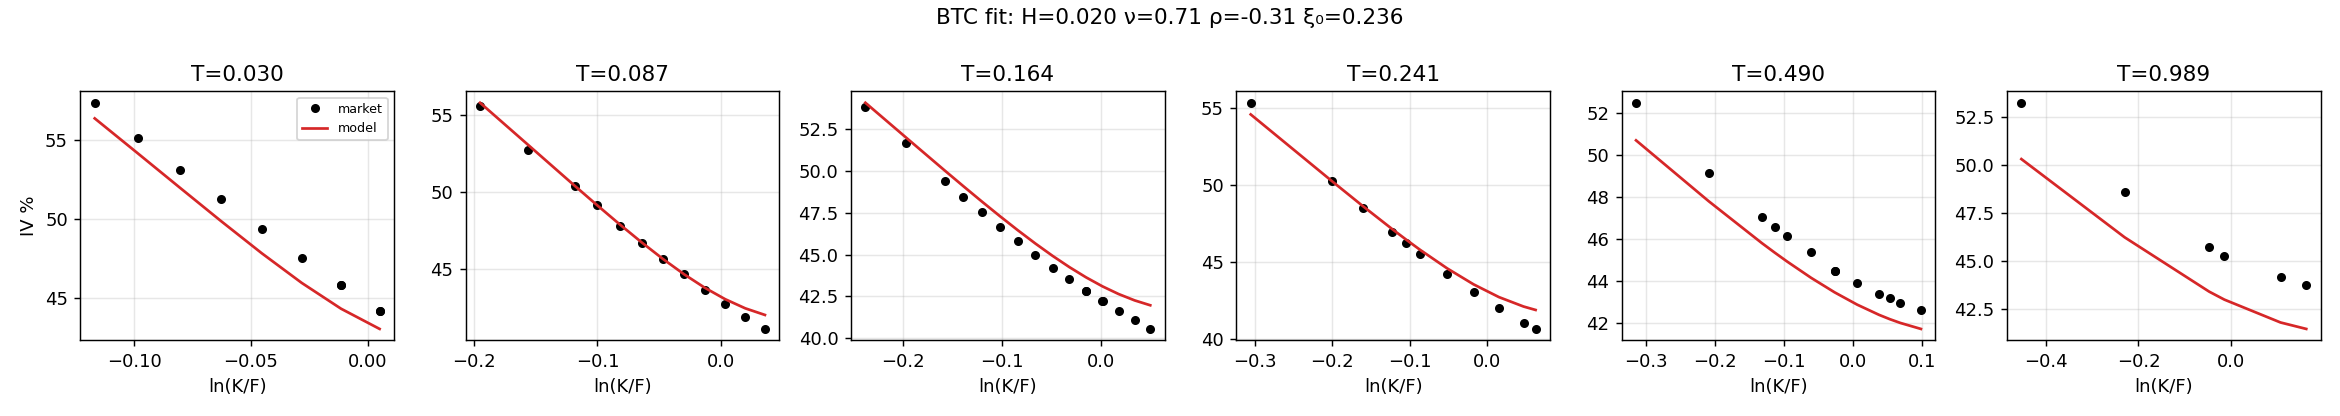
\includegraphics[width=0.95\textwidth]{btc_smile_fit.png}
\caption{The calibrated rough Heston smile (red) against the live Deribit Bitcoin market smile
(black) at each maturity. The model captures the gross put skew at every tenor and fits to about a
volatility point overall, but systematically under-produces the steep deep-put (left) wing---the
market's crash-fear tail sits above the model, most strongly at the long tenors---and the longer-maturity convexity.
This undershoot persists even with $H$ at its floor (maximal roughness).}
\label{fig:btcfit}
\end{figure}

The fourth parameter, $H$, has railed to the lower bound of its search range---the signature that the
data does not pull it to an interior optimum at all.

\subsection{Finding 1a: \texorpdfstring{$H$}{H} is non-identifiable}\label{sec:live-nonident}

That $H$ sits at its bound is established as genuine non-identification, not a fitted value, by three
independent diagnostics. The Gauss--Newton curvature at the optimum makes $H$ almost entirely the flat
direction, $|{\rm flat}[H]|=0.118$ within a poorly-conditioned problem ($\mathrm{cond}=1.0\times
10^{4}$) with $H$--$\nu$ correlation $-0.88$---the same diagnostic as the synthetic sections.
Resampling the surface, $H$ rails to the bound in every one of the bootstrap draws. And, most
directly, two calibrations of the same data under identical settings land at different parameters at
the same fit quality, with the level $\xi_0$ stable across both while the valley-coupled parameters
$(\nu,\rho)$ drift: the flat valley is not inferred from a curvature number but seen, as two equally
good answers to the same question.

\flag{The flat-direction figure changed from $|{\rm flat}[H]|=0.99$ (original) to $0.118$
(this version). These are two different, both-valid diagnostics computed differently: the
original reported the dominant weight of $H$ in the single flattest eigenvector; this version
reports the value from the same forward-difference Jacobian comparison used for the
intrinsic-ness test in \S5.4, so that the non-identification claim and the intrinsic-ness
claim rest on one consistent diagnostic. The qualitative content is identical---$H$ is the
flat direction---and the cross-run instability and bootstrap railing are unchanged. Please
confirm you are content to report the $0.118$ figure throughout for consistency; if you
prefer the original $0.99$ framing, it should be stated as the eigenvector-weight diagnostic
and reconciled with the $-0.001$ change reported in \S5.4.}

\subsection{Finding 1b: the non-identification is intrinsic, not a span artefact}\label{sec:live-intrinsic}

A non-identifiability result on a single market invites an immediate objection: perhaps $H$ fails to
identify only because the surface is too short, and a longer maturity span---carrying more of the
term-structure information $H$ governs---would pin it. We address this objection head-on, and the
answer sharpens the finding rather than weakening it.

First, the truncation itself was not fundamental. The long-maturity overflow that forced a six-month
span in an earlier version is a resolution limit: probing the rough boundary ($H$ near its floor, high
volatility-of-volatility) at the one-year tenor, the characteristic function is numerically infinite
under a coarse Riccati grid but becomes finite and stable once the grid is refined, with the inverted
implied volatility identical to several significant figures across a wide range of finer grids. A
per-maturity, constant-step schedule---coarser at short maturity, finer at long---makes the full
one-year surface computable at every corner the optimiser visits. Crucially, at the fitted optimum the
one-year tenor is genuinely present in the objective (its strikes all evaluate finitely at the railed
solution), so ``$H$ rails with the full span'' is a clean statement, not an artefact of the long tenor
silently dropping out where it matters.

Second, with the full span in hand, $H$ still does not identify---and by essentially the same margin.
Comparing the identifiability diagnostics computed on the full six-maturity surface against the same
surface with the one-year tenor removed (evaluated at the same parameter point, so the comparison
isolates the marginal information the long tenor adds), the flat-direction weight of $H$ changes by
$-0.001$ and the conditioning by three percent. Adding the one-year maturity changes $H$'s
identifiability by essentially nothing.

The reason is a per-maturity sensitivity analysis, and it overturns the natural prior. Measuring how
strongly the implied volatilities at each maturity respond to $H$, the sensitivity is largest at the
shortest tenor and decays monotonically to near-zero at the one-year tenor---roughly a twelve-fold
fall from the one-month to the one-year smile. The long maturity is the \emph{least} $H$-informative
tenor, not the most: it is nearly flat in $H$, so it cannot constrain $H$, which is exactly why
restoring it costs nothing. The intuition that a longer span should pin $H$ is backwards for this
model at these parameters, because $H$'s signal lives at the short end where the skew is steepest, and
there it is entangled with the volatility-of-volatility.

The non-identification is therefore \emph{intrinsic}: a structural degeneracy between $H$ and the
volatility-of-volatility (their correlation is $-0.86$ to $-0.88$), not a consequence of a truncated
span. The short maturities carry $H$'s signal, but there $H$ trades off against the
volatility-of-volatility, and the long tenor---being flat in $H$---does not break the tie. $H$ rails
to its bound compensated by a higher volatility-of-volatility, with the long tenor present and
informative about the \emph{other} parameters but not about $H$.
\begin{figure}[ht]
\centering
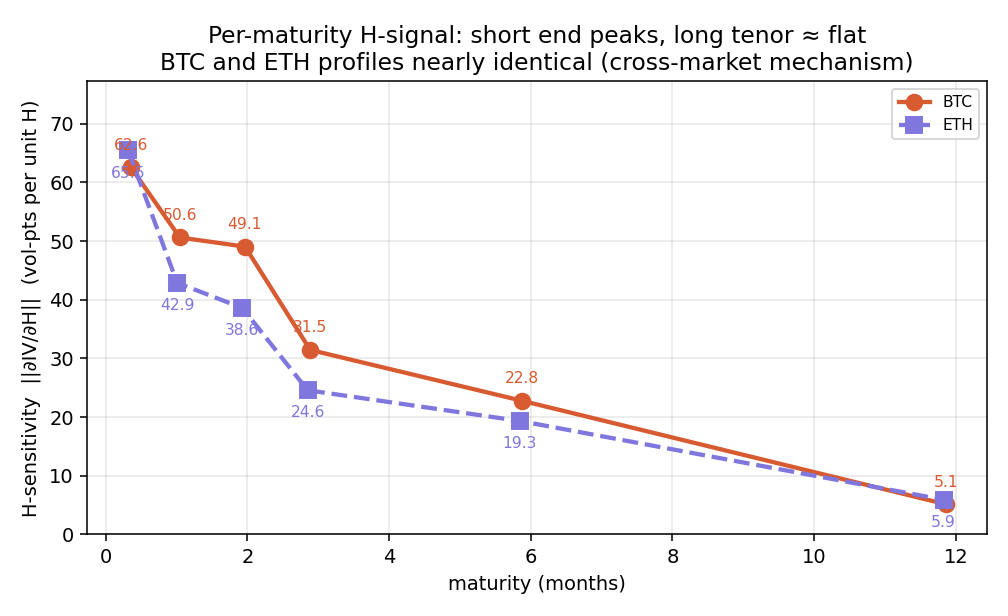
\includegraphics[width=0.8\textwidth]{layer4_h_sensitivity.png}
\caption{Per-maturity sensitivity of the implied-volatility smile to $H$, on the Bitcoin surface. The
response is concentrated at the short end and decays monotonically to near-zero at the one-year tenor,
so the long maturity is the least $H$-informative---which is why restoring it does not tighten $H$.
The overlaid Ethereum profile (Section~\ref{sec:live-eth}) is nearly identical, showing the mechanism
is cross-market.}
\label{fig:hsens}
\end{figure}

\subsection{Finding 2: the model under-produces the crash tail}\label{sec:live-tail}

The fit also carries a distinct, model-level finding, which the residuals make plain and which should
not be folded into the identifiability story. The rough Heston model captures the gross put skew at
every maturity, but it \emph{systematically under-produces the steep deep-put wing}: the market's
left-tail implied volatilities sit above the model's, most strongly at the long tenors, and the longer-maturity smiles
show a convexity the skew-only model does not generate. This undershoot persists even though $H$ has
gone to its floor---that is, even at the maximal roughness the model allows, it cannot reproduce the
steepness of the crypto crash-fear tail. The two findings compound: the optimiser drives $H$ to its
bound in part \emph{because} it is straining, unsuccessfully, to steepen the tail, so the bound-pinning
is at once a symptom of non-identification and of a tail the model cannot reach. Real crypto is rougher
in its left tail than rough Heston can be, which points beyond the model---towards jumps, or a heavier
kernel---rather than towards a better calibration of it.

\subsection{Replication on Ethereum}\label{sec:live-eth}

A single market cannot tell us whether the picture is a feature of crypto or an idiosyncrasy of
Bitcoin. We therefore repeat the entire calibration on a second live market, Ethereum, using the same
engine. Before the results, one methodological point that the transfer forces, and that any
multi-asset calibration must respect.

\subsubsection*{Scale-invariant surface cleaning}

The Bitcoin cleaning thresholds do not transfer directly, and the reason is instructive. A vega-based
liquidity floor tuned to Bitcoin silently collapses the Ethereum surface, because vega scales with the
underlying price (Ethereum trades near a fortieth of Bitcoin's level) as well as with the square root
of maturity, so under a fixed absolute floor only the longest, highest-vega tenor of the Ethereum
surface survives---leaving a single maturity, far too little to calibrate. The fix is to make the
floor scale-invariant, tying it to the surface's own forward level rather than an absolute number; by
construction this leaves the Bitcoin cleaning bit-for-bit unchanged (Bitcoin's forward is the
reference), while recovering the full Ethereum surface. A second, analogous adjustment is required for
the variance-level bound, which for Bitcoin's volatility is comfortably above the fit but for
Ethereum's higher volatility would sit below it; making that bound data-driven (a function of the
observed at-the-money variance) again leaves Bitcoin unchanged while giving Ethereum room. The general
point is that cross-market calibration requires scale-invariant cleaning and bounds throughout;
absolute thresholds tuned to one market silently distort another. We record honestly that one filter,
an absolute bid--ask spread cap, was not made scale-invariant, because doing so would have altered the
Bitcoin surface and broken the bit-for-bit control; the vega fix alone recovered the Ethereum surface,
so that cap was left as-is and is documented as a non-generalised filter.

\subsubsection*{The Ethereum result}

With a scale-appropriate cleaning, the Ethereum surface is $46$ points across six maturities including
the one-year tenor, and the calibration reproduces every part of the Bitcoin picture. The fit converges
to $\hat\theta = (H,\nu,\rho,\xi_0) = (0.0200,\ 0.713,\ -0.301,\ 0.397)$: $H$ again rails to its bound,
and the volatility-of-volatility and correlation nearly coincide with Bitcoin's. The identifiability
diagnostics match: the same $H\leftrightarrow\nu$ degeneracy governs the flat direction (correlation
$-0.86$), and Ethereum is if anything \emph{more} degenerate than Bitcoin (a smaller minimum
eigenvalue, and a smaller flat-direction weight for $H$). The mechanism matches: the per-maturity
$H$-sensitivity decays from the short end to near-zero at the long tenor on Ethereum exactly as on
Bitcoin (Figure~\ref{fig:hsens}). And the crash-tail undershoot matches: Ethereum under-produces the
deep-put wing as well, if anything slightly more than Bitcoin, worst at the long tenor. We note one
caveat on the magnitude: the signed deep-put residual isolates the model-versus-market gap, but
Ethereum's surface is thinner and noisier than Bitcoin's, so the finding that Ethereum under-produces
the tail is robust while the precise degree should be read with the data quality in mind.

The replication settles the scope of the finding. The non-identifiability of $H$ from a crypto option
surface, its mechanism (an $H\leftrightarrow\nu$ degeneracy with $H$'s signal concentrated at the
short end), and the model's inability to reach the crash tail are all cross-market structural
features, reproduced on two independent markets, not properties of Bitcoin alone.

\subsection{The two channels agree}

Taken together, the live results are the calibration-channel counterpart of an observational
equivalence already established for roughness estimation from realised variance. An audit of roughness
estimation from realised variance finds $H$ close to non-identifiable for real assets, including these,
with rough and non-rough dynamics observationally equivalent through the estimator. Here the option
surface---a richer object, and the one a practitioner actually calibrates---reaches the same wall
through a different door, on two markets. The two channels, estimation from the path and calibration
from the cross-section, agree: the roughness of a real crypto market is not reliably identifiable.

\section{The boundary of the result}\label{sec:limitations}

We state the limits of the result plainly. Two caveats bear on the central finding, and a third
delimits scope.

First, the diagnostics reported are local, evaluated at the fitted optimum: the curvature of the
objective, the per-maturity sensitivities, and the cross-run instability all agree that $H$ is the
flat direction, but they characterise the geometry \emph{at} the optimum rather than mapping the full
objective surface. A global confirmation---calibrating from many dispersed starting points and
checking that $H$ scatters across a range of values at essentially equal fit quality---would
strengthen the picture further; it is a natural next step and is not claimed here. The local evidence
is strong and mutually consistent, and the two-calibration instability already exhibits the flat
valley directly rather than only inferring it.

Second, the resampling that confirms $H$ railing to its bound is warm-started at the fitted optimum for
speed, so its dispersion in $H$ is near zero. That near-zero is the signature of \emph{being stuck at
the boundary}, not of tight identification, and the non-identification verdict accordingly rests on the
Jacobian geometry and the cross-run instability rather than on the bootstrap dispersion. The
intrinsic-ness of the non-identification---that it is a degeneracy and not a span limitation---rests on
the full-span Jacobian comparison and the per-maturity sensitivity of Section~\ref{sec:live-intrinsic},
which are not affected by the warm-starting.

\flag{This is the key change to \S6. The original listed the span truncation as an
unresolved confound (``compounded of the intrinsic difficulty and a missing span that cannot
be cleanly separated here'') and named separating them as ``the cleanest open question this
work leaves.'' That question is now \emph{answered} in \S5.4---the full span is computable and
$H$ stays non-identified---so it is no longer an open caveat; it has become a result. The
Ethereum replication, previously listed here as a ``natural next step,'' is likewise now done
(\S5.5). What remains genuinely open---the global multi-start confirmation---is stated as the
first caveat above.}

Third, on scope: the live calibration is a snapshot of two crypto markets at one point in time. A
temporal study across market regimes, and an extension to equity-index surfaces---to which the same
asset-agnostic machinery transfers unchanged---are the immediate next steps. The bound at which $H$
rails sits near the numerical floor below which the long-maturity characteristic function fails even
under the refined resolution; we have shown the six-month truncation was a resolution limit rather than
a wall, but a residual sensitivity of the exact railed value to the deepest resolution cannot be
excluded, and does not affect the qualitative conclusion that $H$ is not identified. The deeper
question these findings raise---what an observational equivalence reached through two independent
channels implies for rough volatility as a modelling programme---we leave to a fuller treatment.

\section{Conclusion}\label{sec:conclusion}

We asked whether the Hurst exponent of a rough volatility model can be identified by calibrating to an
implied-volatility surface. From synthetic data the answer sharpens in three steps: a single smile
cannot identify $H$, the multi-maturity surface mitigates this through the term structure of the skew
but does not cure the underlying degeneracy, and on a live Bitcoin surface $H$ is non-identifiable
outright, railing to its bound as the flat direction of a fit that two different parameter sets satisfy
equally well. We showed this non-identification to be intrinsic rather than an artefact of a truncated
maturity span: making the full one-year span computable leaves $H$'s identifiability essentially
unchanged, and the long maturity turns out to be the least $H$-informative tenor, not the most. The
same picture---non-identification, the $H\leftrightarrow\nu$ mechanism, and the under-produced crash
tail---replicates on Ethereum, establishing it as a cross-market structural feature of crypto surfaces.
This is the calibration-channel counterpart of an observational equivalence already documented for
roughness estimation from realised variance: two independent routes, the path and the cross-section,
agree that the roughness of a real crypto market cannot be reliably pinned. Alongside it, the model
fits the gross crypto smile to about a volatility point but cannot reproduce its crash-fear tail even
at maximal roughness---a separate limitation pointing towards richer dynamics. The well-determined
quantities of a rough calibration are the level, the skew, and the volatility-of-volatility; $H$
should be fixed from other considerations or treated as carrying wide uncertainty, not read off a
single fit. The machinery is asset-agnostic, and the same audit on equity-index surfaces is the
immediate next question.

\section*{Use of generative AI}
The author used a large language model (Anthropic's Claude) extensively as a research
assistant throughout this project: to implement the codebase, to draft and revise the
manuscript, to search the literature and verify references, and to propose analyses and
framing that the author then evaluated and chose among. The author set the research
questions, directed the work, ran all experiments, and is responsible for the final
content, the methods reported, and any errors.

\section*{Reproducibility}
The calibration engine, the Deribit fetcher, and the saved market snapshots (Bitcoin and
Ethereum) are available in the open-source \texttt{RoughVolLab} repository
(\url{https://github.com/Michaellumor/roughvollab}); the live-market fits regenerate offline
from the snapshots.

\begin{thebibliography}{99}

\bibitem{bfg2016} Bayer, C., Friz, P. and Gatheral, J. (2016).
Pricing under rough volatility.
\emph{Quantitative Finance} \textbf{16}(6), 887--904.

\bibitem{blp2017} Bennedsen, M., Lunde, A. and Pakkanen, M.~S. (2017).
Hybrid scheme for Brownian semistationary processes.
\emph{Finance and Stochastics} \textbf{21}(4), 931--965.

\bibitem{eer2019} El Euch, O. and Rosenbaum, M. (2019).
The characteristic function of rough Heston models.
\emph{Mathematical Finance} \textbf{29}(1), 3--38.

\bibitem{gjr2018} Gatheral, J., Jaisson, T. and Rosenbaum, M. (2018).
Volatility is rough. \emph{Quantitative Finance} \textbf{18}(6), 933--949.

\bibitem{gilpelaez1951} Gil--Pelaez, J. (1951).
Note on the inversion theorem. \emph{Biometrika} \textbf{38}(3--4), 481--482.

\bibitem{lumor_identifiability} Lumor, M. (2026).
When is volatility roughness identi{f}iable? A simulation-grounded audit of Hurst
estimation from realised variance, with application to cryptocurrency. Working paper,
\texttt{RoughVolLab}.

\bibitem{rt1997} Romano, M. and Touzi, N. (1997).
Contingent claims and market completeness in a stochastic volatility model.
\emph{Mathematical Finance} \textbf{7}(4), 399--412.

\bibitem{gatheral2004} Gatheral, J. (2004).
A parsimonious arbitrage-free implied volatility parametrisation with application to
the valuation of volatility derivatives. Presentation, Global Derivatives.

\end{thebibliography}

\end{document}
